\chapter{Diseño}
En esta sección se describirá el diseño de la plataforma \textbf{GAC} (Gestor Académico de Calendarios). Se detallarán los aspectos más relevantes de la arquitectura, la interfaz de usuario y la base de datos.

\newpage

\section{Arquitectura software}
La arquitectura software se refiere a la vista del sistema que incluye los componentes principales del mismo, la conducta de dichos componentes según se la percibe desde el resto del sistema y las formas en las que interactúan y se coordinan entre sí para lograr los objetivos del sistema. Sus dos principales aspectos son, que provee de un plan de diseño, un ``blueprint'' del sistema a la vez que hace de abstracción del mismo para ayudar a manejar la complejidad del mismo. Una buena arquitectura software es el garante de un sistema que cumple con los requisitos de calidad, como la eficiencia, la fiabilidad, la seguridad, la mantenibilidad, la escalabilidad, la portabilidad, la usabilidad, la interoperabilidad, la disponibilidad y la capacidad de evolución \cite{hofmeister2000applied, reynoso2004introduccion, garlan2008software}.\newline

Para el desarrollo de la plataforma se ha optado por una arquitectura cliente-servidor basada en una arquitectura orientada a servicios (SOA). La API\footnote{\url{https://aws.amazon.com/es/what-is/api/}} ha sido desarrollada en Python y Flask y se encarga de manejar las solicitudes del cliente.\newline

Adicionalmente, se ha desarrollado un web scraper\footnote{\url{https://kinsta.com/es/base-de-conocimiento/que-es-web-scraping/}} que se encarga de obtener toda la programación docente de la oficina virtual de la Universidad de Granada\footnote{\url{https://oficinavirtual.ugr.es}}. Los usuarios realizan peticiones desde la plataforma web al servidor, el cual se encarga de procesarlas y devolver una respuesta.\newline

\subsection{Arquitectura Orientada a Servicios (SOA)}

La Arquitectura Orientada a Servicios\footnote{\url{https://www.redhat.com/es/topics/cloud-native-apps/what-is-service-oriented-architecture}} es un tipo de diseño de software que permite reutilizar sus elementos gracias a las interfaces de servicios que se comunican a través de una red con un lenguaje común. Un servicio es una unidad autónoma de una o más funciones software, diseñada para realizar una tarea específica, como recuperar cierta información o ejecutar una operación. Dado que SOA expone los servicios utilizando protocolos estándar de red para enviar solicitudes o acceder a los datos, se facilita la interoperabilidad entre diferentes sistemas y la atomicidad desde la perspectiva del usuario \cite{laskey2009service, 1210138}.\newline

Bajo el marco de una arquitectura cliente-servidor, las llamadas a los servicios se realizan mediante el protocolo HTTP y la información de respuesta se devuelve en formato JSON, estándar en la intercomunicación de esta arquitectura.\newline

\begin{figure}
    \centering
    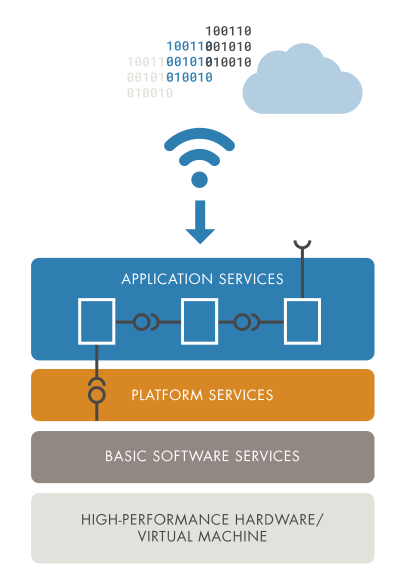
\includegraphics[width=0.5\textwidth]{./imagenes/SOA.png}
    \caption{Pila de software SOA generalizada \cite{soa}.}
\end{figure}

\section{Tecnologías Utilizadas}

Para el desarrollo de la plataforma se compone de un backend y un frontend. El backend hace de servidor y es el que se encarga de responder a las peticiones por medio de una API desarrollada en Python con Flask y SQLite como base de datos. El frontend incluye la interfaz de usuario y ha sido desarrollada en ReactJS. A continuación se detallan las tecnologías utilizadas en detalle.

\subsection{Desarrollo Backend}

El backend es el encargado de administrar la funcionalidad general de la plataforma, operando en el servidor para procesar las solicitudes, manipular los datos y devolver la respuesta al cliente. En esta capa se almacena el código encargado de la lógica de negocio y la interacción con la base de datos. Su funcionalidad juega un papel esencial en la comunicación con el frontend y se asegura de que la información devuelta sea correcta, asegurando la integridad de los datos, el dinamismo y el diseño responsive de la interfaz de usuario. Actuando como núcleo funcional de la plataforma, se compone de las tecnologías que se detallan a continuación.

\subsubsection*{Python}
Es un lenguaje de programación interpretado, orientado a objetos y de alto nivel con semántica dinámica. Su sintaxis es clara y legible, lo que facilita la escritura de código y la lectura del mismo. Es un lenguaje multiplataforma, lo que significa que se puede ejecutar en cualquier sistema operativo. Es versátil y se puede utilizar en una amplia variedad de aplicaciones, desde desarrollo web hasta análisis de datos y aprendizaje automático. Es un lenguaje de programación muy popular y cuenta con una gran cantidad de bibliotecas y marcos de trabajo que facilitan el desarrollo de aplicaciones \cite{python2021python}.\newline

El motivo de usar Python para el desarrollo del backend se debe a una elección personal, motivada por el interés de aprender un nuevo lenguaje de programación tan ampliamente utilizado a nivel mundial. Python es reconocido por su simplicidad y facilidad de uso, lo que lo convierte en una excelente opción para el desarrollo de aplicaciones web. Cuenta con una gran cantidad de bibliotecas y marcos de trabajo que facilitan el desarrollo de aplicaciones web, la documentación es extensa y la comunidad es muy activa y además soporta módulos y paquetes que lo que resulta en productos modulares y reutilizables.

\subsubsection*{Flask}
Es un framework de aplicaciones web escrito en Python. Se compone de un núcleo WSGI\footnote{\url{https://wsgi.readthedocs.io/en/latest/}} simple y fácil de extender que permite a los desarrolladores crear aplicaciones web rápidamente con una mínima configuración. Flask\footnote{\url{https://pythonbasics.org/what-is-flask-python/}} es ligero y fácil de usar, lo que lo convierte en una muy buena opción para desarrollar proyectos de pequeños o medianos. Es muy popular y cuenta con una gran cantidad de bibliotecas y extensiones que facilitan el desarrollo \cite{grinberg2018flask}.\newline

La recomendación de usar Flask vino por parte de mi tutor, ya que es un framework muy popular, modular y fácil de usar. En la red hay disponibles una gran cantidad de guías que explican los pasos necesarios para hacer una configuración inicial y empezar a desarrollar aplicaciones. Dada la familiaridad con este framework y su baja curva de aprendizaje, se decidió utilizar para el desarrollo del backend.

\subsubsection*{SQLite}

SQLite\footnote{\url{https://www.sqlite.org/index.html}} es una base de datos relacional embebida, de código abierto, que se implementa como una biblioteca de programación C. Es rápida, ligera y fácil de usar, lo que la convierte en una excelente opción para aplicaciones de pequeña o mediana envergadura. Es muy popular y cuenta con una gran cantidad de bibliotecas y extensiones que facilitan el desarrollo \cite{kreibich2010using}.\newline

La elección de SQLite como base de datos se debe a que es una base de datos embebida, lo que significa que no requiere un servidor de base de datos separado para funcionar. Esto simplifica la configuración y el despliegue de la plataforma. Además, es de tipo relacional, y dada la estructura rígida de asignaturas, grupos, subgrupos, aulas, etc., se ajusta perfectamente a las necesidades de la plataforma. Por último, es muy fácil de usar y cuenta con una gran cantidad de bibliotecas y extensiones que facilitan el desarrollo, como es el caso de \textbf{SQLAlchemy}\footnote{\url{https://www.sqlalchemy.org/}} que usaremos para facilitar la interacción con la base de datos.

\subsubsection*{Docker}

Docker \footnote{\url{https://www.docker.com/}} es una tecnología de organización de contenedores que permite empaquetar aplicaciones en contenedores virtuales que pueden ejecutarse en cualquier lugar. Provee un tipo de virtualización más ligera que las máquinas virtuales tradicionales, ya que comparte el núcleo del sistema operativo con otros contenedores.\newline

El motivo de usar Docker es mi familiaridad con la herramienta y mi interés en aprender más sobre ella. Docker es una tecnología muy popular y ampliamente utilizada en la industria. Permite empaquetar aplicaciones en contenedores virtuales que pueden ejecutarse en las mismas condiciones independientemente del sistema operativo subyacente, lo que facilita la configuración y el despliegue de la plataforma. Además, es muy eficiente y ligero, permitiendo ejecutar múltiples contenedores en un mismo servidor.

\subsection{Desarrollo Frontend}

El frontend es la parte de la plataforma con la que interactúan los usuarios finales. Es la capa de presentación e incluye todo aquello que el se ve. Juega un papel fundamental en la experiencia ya que es la primera impresión que se lleva el usuario y debe ser clara e intuitiva.\newline

\subsubsection*{ReactJS}

ReactJS\footnote{\url{https://es.reactjs.org/}} es una biblioteca de JavaScript de código abierto diseñada para crear interfaces de usuario interactivas, modulares y reutilizables. Permite el desarrollo de aplicaciones web que cambian sus datos sin necesidad de recargar la página. Provee un DOM mucho más eficiente y ligero almacenado en memoria y con el que interactúa en lugar de hacerlo directamente con el DOM del navegador. En la mayoría de webframeworks, se manipula el DOM completamente en cada uno de los eventos que desencadena la página, como consecuencia de esto, en los casos en los que se modifica una gran cantidad de datos, el rendimiento se ve seriamente afectado. ReactJS soluciona este problema, ya que solo modifica los elementos que han cambiado, haciendo uso de lo que se conoce como Virtual DOM\footnote{\url{https://es.reactjs.org/docs/faq-internals.html}}. Es muy popular y cuenta con una gran cantidad de bibliotecas y extensiones que facilitan el desarrollo \cite{aggarwal2018modern}.\newline

La utilización de ReactJS se debe a que es una biblioteca de JavaScript muy popular y ampliamente utilizada en la industria. Es muy eficiente y permite el desarrollo de aplicaciones web interactivas y modulares. Además, sirve de base para el desarrollo de aplicaciones móviles con React Native\footnote{\url{https://reactnative.dev/}}.\newline

Para ilustrar su popularidad, a continuación se muestra un gráfico con las tendencias de NPM\footnote{\url{https://npmtrends.com/@angular/core-vs-angular-vs-react-vs-vue}} que pese a no ser una fuente totalmente fiable (podemos ver un pico de Vue en la gráfica que puede haberse hecho por error o maliciosamente para alterar las estadísticas), nos da una idea de la popularidad de ReactJS en la actualidad.

\begin{figure}[H]
    \centering
    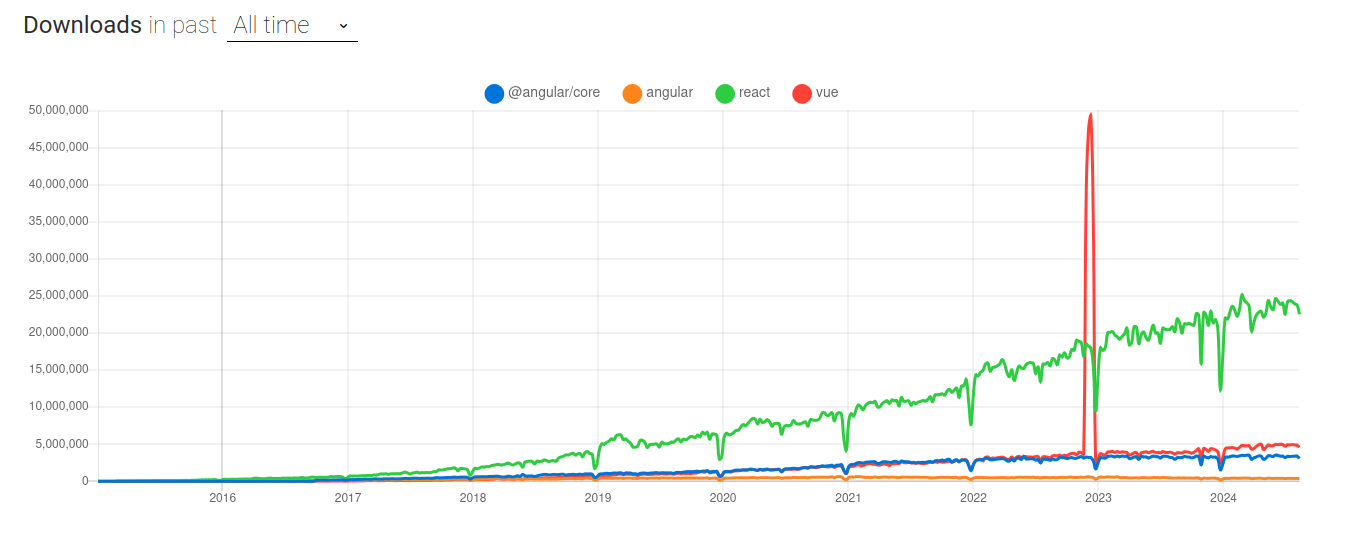
\includegraphics[width=1\textwidth]{./imagenes/Comparativa.png}
    \caption{Comparativa de descargas de frameworks de acuerdo a NPM.}
\end{figure}

\newpage

\subsection{Herramientas de Desarrollo}

\newcommand{\icon}[1]{\includegraphics[height=18pt]{#1}}
\subsubsection*{Visual Studio Code \protect\icon{./imagenes/vscode_logo.png}}

Visual Studio Code\footnote{\url{https://code.visualstudio.com/}} es un editor de código fuente desarrollado por Microsoft para Windows, Linux y macOS. Dispone de características como resaltado de sintaxis, finalización de código, refactorización de código, depuración, control de versiones, entre otras. Soporta una gran cantidad de lenguajes de programación y cuenta con una gran cantidad de extensiones que facilitan el desarrollo. \newline

La razón principal de la elección de Visual Studio Code es la familiaridad. He utilizado este editor desde que empecé mis estudios de grado y la personalización, extensiones, integración con Git y la facilidad de uso la hacen una herramienta tremendamente útil y versátil. Además, pueden integrarse terminales para ejecutar comandos y es multiplataforma, lo que permite trabajar en cualquier sistema operativo.\newline

\renewcommand{\icon}[1]{\includegraphics[height=18pt]{#1}}
\subsubsection*{SQLite Studio \protect\icon{./imagenes/sqlite_logo.png}}


SQLite Studio\footnote{\url{https://sqlitestudio.pl/}} es un administrador de bases de datos multiplataforma que permite navegar y editar archivos de bases de datos SQLite. Dispone de características como la creación de bases de datos, tablas, índices, vistas, procedimientos almacenados, funciones, etc. Además, permite ejecutar consultas SQL, importar y exportar datos, entre otras.\newline

La elección de SQLite Studio se debe a que es un administrador de bases de datos muy completo y fácil de usar. Permite gestionar varias bases de datos SQLite de forma sencilla y eficiente, lo que facilita el desarrollo y la depuración.\newline

\begin{figure}[H]
    \centering
    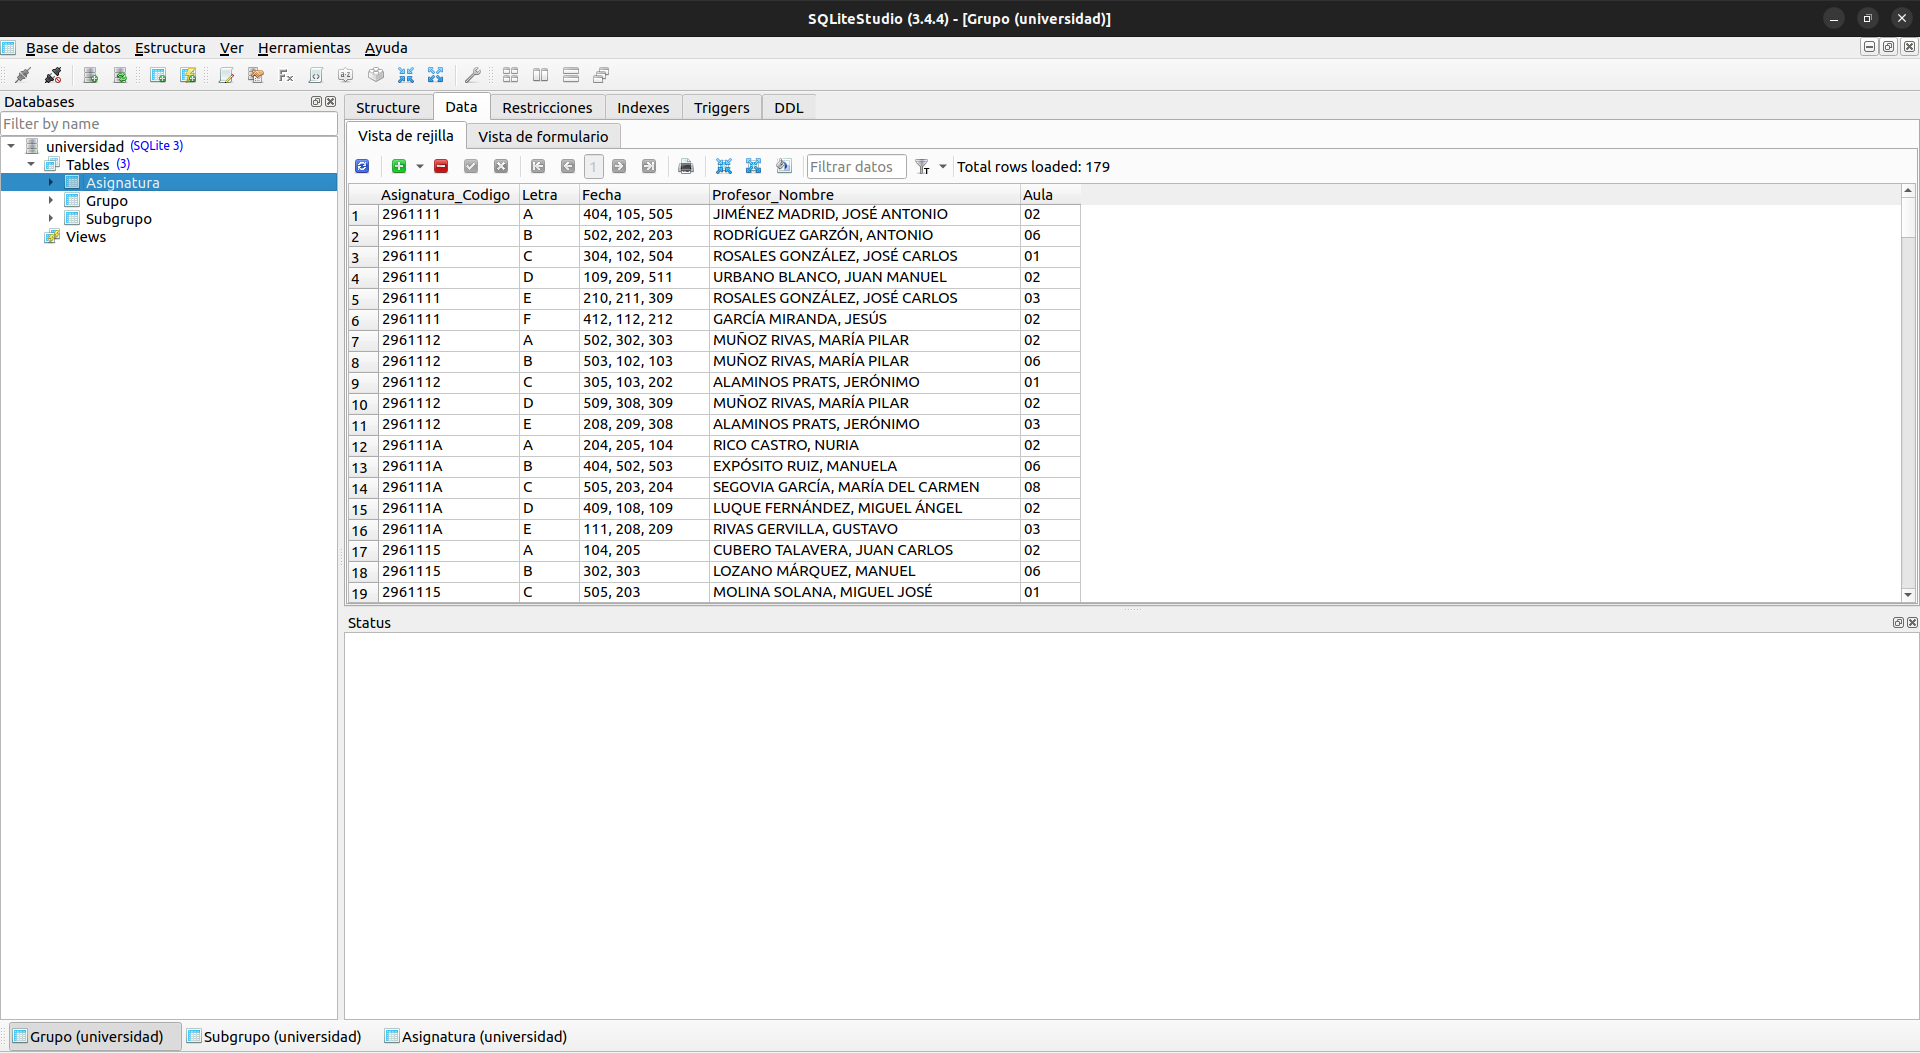
\includegraphics[width=1\textwidth]{./imagenes/SQLiteStudio.png}
    \caption{SQLite Studio.}
\end{figure}

\renewcommand{\icon}[1]{\includegraphics[height=18pt]{#1}}
\subsubsection*{Postman \protect\icon{./imagenes/postman_logo.png}}



Postman\footnote{\url{https://www.postman.com/}} es una plataforma para crear y utilizar API. Simplifica cada paso del ciclo de vida de una API y agiliza el desarrollo. Permite enviar solicitudes HTTP a un servidor y recibir respuestas. Dispone de características como la creación de \textit{colecciones de solicitudes}, la automatización de pruebas, la documentación de la API, entre otras. Es muy popular y cuenta con una gran cantidad de usuarios en todo el mundo.\newline

La elección de Postman se debe a una recomendación de mi tutor. Es una herramienta muy útil para probar API y asegurarse de que funcionan correctamente. Gracias a ella he podido probar los datos cruzados entre el backend y el frontend y depurar de manera más cómoda. Además, permite automatizar las pruebas y documentarlas.\newline

\renewcommand{\icon}[1]{\includegraphics[height=8pt]{#1}}
\subsubsection*{Textidote \protect\icon{./imagenes/textidote_logo.png}}



Textidote\footnote{\url{https://sylvainhalle.github.io/textidote/}} es un corrector ortográfico y gramatical de código abierto. Dispone de características como el resaltado de errores ortográficos y gramaticales, la sugerencia de sinónimos, la detección de frases redundantes, entre otras. Es muy útil para mejorar la calidad del código y evitar errores comunes. Fue diseñado para trabajar específicamente sobre Latex\newline

El motivo de la elección de esta herramienta fue para poder revisar el código de la documentación en LaTeX de este proyecto. Dado que el código contiene comandos especiales y palabras clave, no es posible aplicar correctores gramaticales comunes, a no ser que se extraiga el texto plano, pero Textidote está desarrollado para trabajar específicamente sobre Latex. Además, cuenta con una gran cantidad de usuarios en todo el mundo lo que hace más fácil encontrar soluciones a problemas comunes.\newline

\section{Diseño Lógico}

Los diagramas de clase UML (Unified Modeling Language) son el núcleo del diseño y analisis orientado a objetos y son una forma de modelar la estructura estática de un sistema, por medio de clases, atributos, métodos y relaciones entre ellas \cite{herchi2012user}.\newline

SQLite ha sido la opción escogida para la base de datos de la plataforma \textbf{GAC}, por los motivos mencionados anteriormente. Todas las clases del diagrama que se muestra a continuación, se traducirán a tablas donde sus campos serán los atributos que se detallan en la figura. A continuación se muestra el diagrama de clases de la plataforma.\newline

\begin{figure}[H]
    \centering
    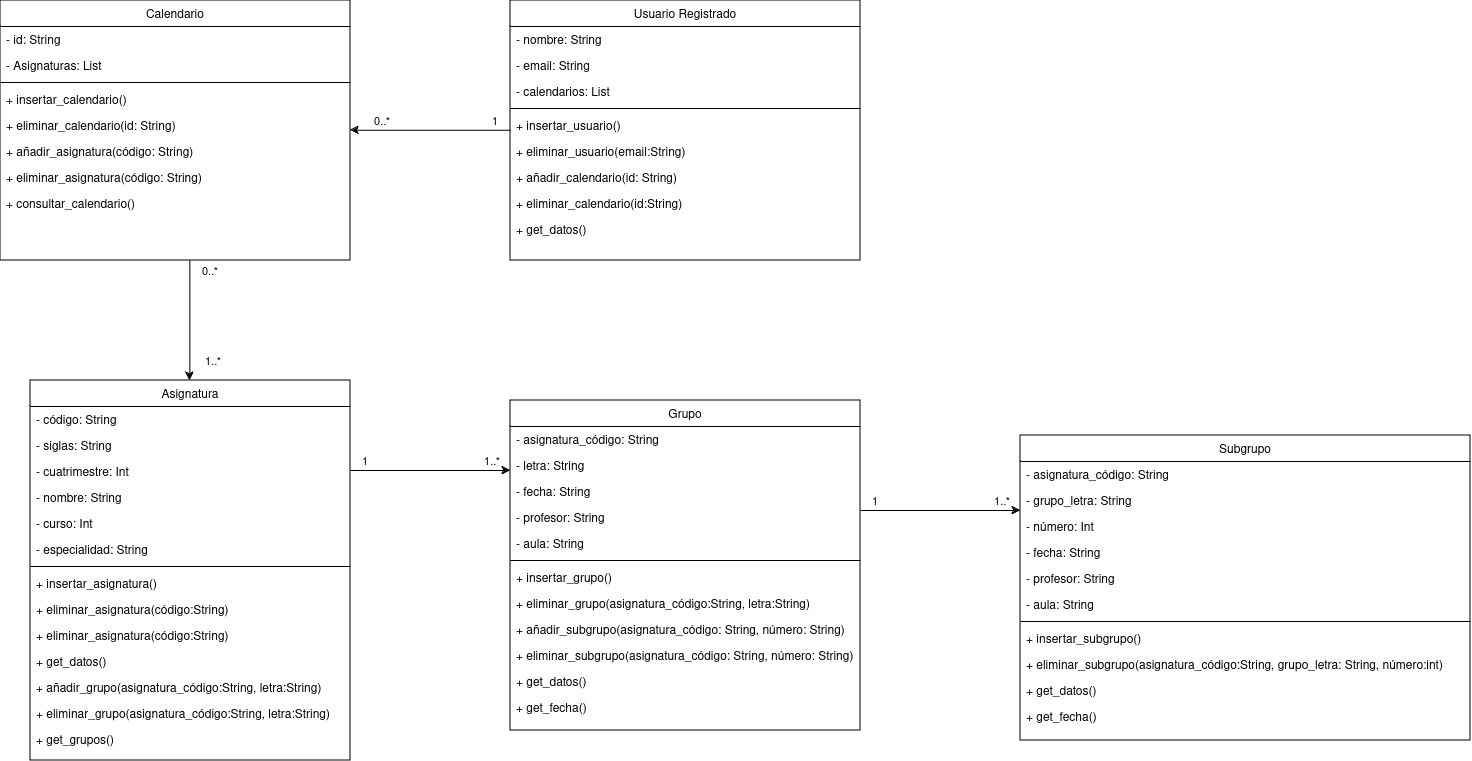
\includegraphics[width=1\textwidth]{./imagenes/Class_Diagram.png}
    \caption{Diagrama de clases de la plataforma.}
\end{figure}


\section{Diseño de Wireframes para Frontend}

Un wireframe\footnote{\url{https://miro.com/es/wireframe/que-es-wireframe/}} es un diagrama visual que esboza el esqueleto de un proyecto o pieza tecnológica. Los diseñadores de UX (User Experience) suelen utilizarlo para trazar el diseño y la composición de su trabajo si entrar en detalles de paletas de color, etc. Es la etapa previa a los mockups y prototipos.\newline

El wireframe que se muestra a continuación, pertenece a los primeros bocetos de la interfaz de usuario de la plataforma \textbf{GAC}. En las primeras etapas del diseño se consideró la opción de emplear un modelo de inteligencia artificial para la generación de los calendarios, además se pretendía que la plataforma fuese una especie de organizador personal tipo Google Calendar. Pueden consultarse el resto de diseños en el anexo I.\newline


\begin{figure}[H]
    \centering
    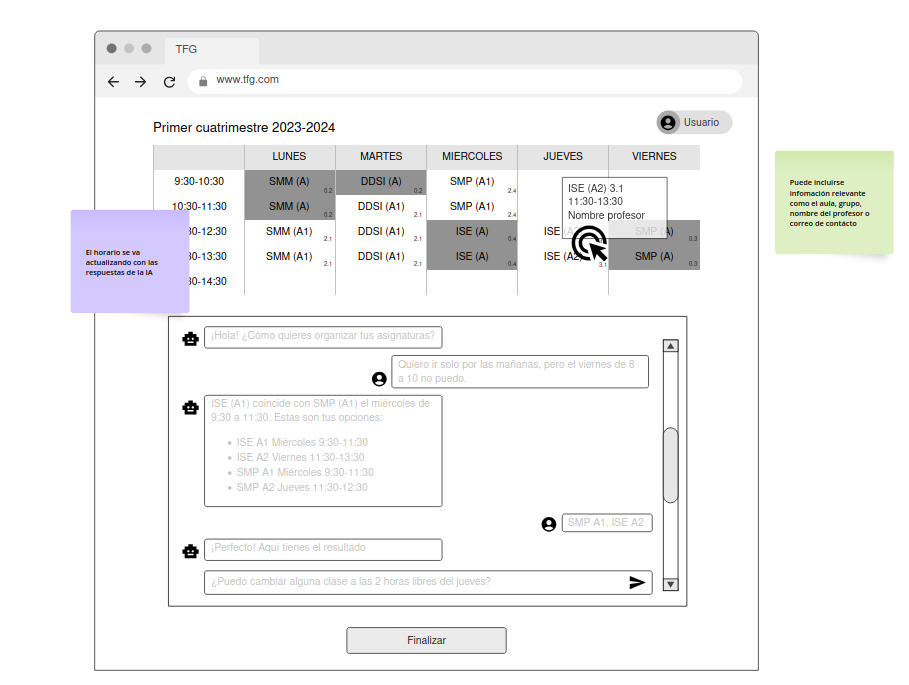
\includegraphics[width=1\textwidth]{./imagenes/Mockup_calendario.png}
    \caption{Calendario con asistente.}
\end{figure}

\begin{figure}[H]
    \centering
    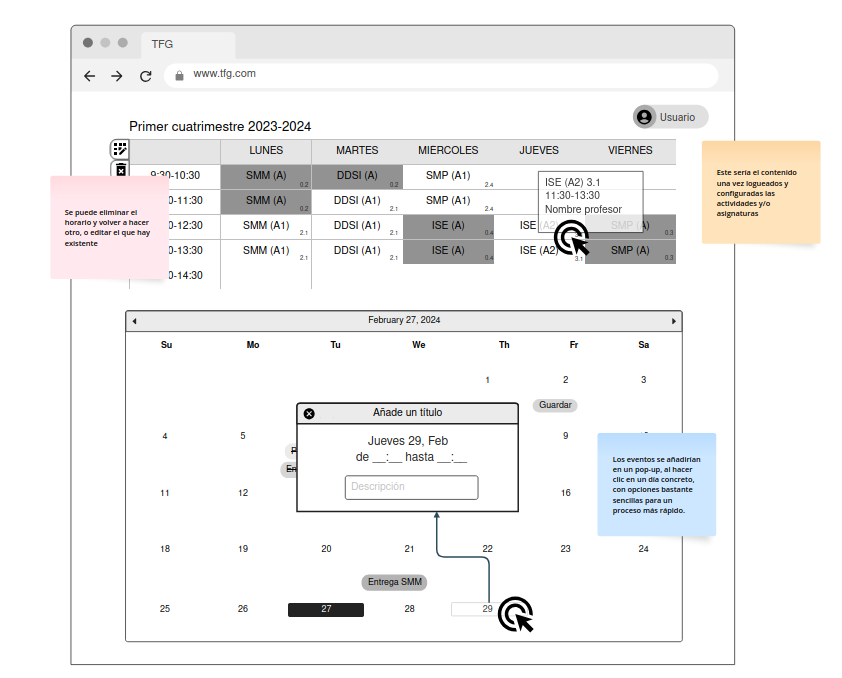
\includegraphics[width=1\textwidth]{./imagenes/Mockup_organizador.png}
    \caption{Calendario académico y mensual de actividades.}
\end{figure}

\begin{figure}[H]
    \centering
    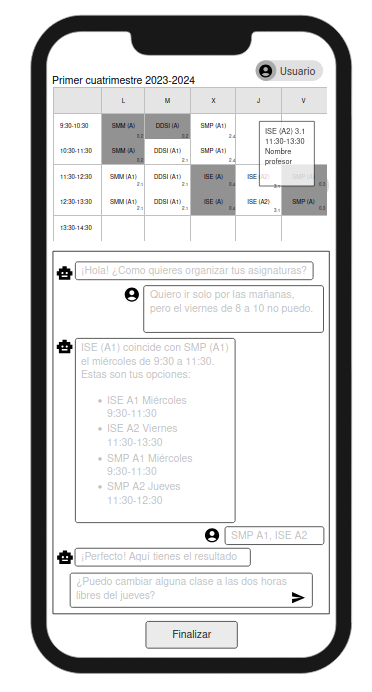
\includegraphics[width=0.3\textwidth]{./imagenes/Mockups_smartphone.png}
    \caption{Calendario con asistente para smartphone.}
\end{figure}


